\documentclass{article}

\usepackage[english]{babel}

\usepackage[a4paper,top=2cm,bottom=2cm,left=3cm,right=3cm,marginparwidth=1.75cm]{geometry}

\usepackage{graphicx}
\usepackage[colorlinks=true, allcolors=blue]{hyperref}

\title{Languages and Algorithms for Artificial Intelligence}

\date{February 2022}
\author{Anna Valanzano, Michele Milesi, Pietro Epis}

\begin{document}
\maketitle

\begin{abstract}
In this paper we reported a short explanation about the programs that we have developed to solve the \href{https://giochimatematici.unibocconi.it/index.php/gare/giochi-d-autunno/170-gli-allenamenti-ai-giochi-d-autunno}{Bocconi mathematical games}. 
Each puzzle has been solved in Minizinc and most of them have been developed also in Prolog.
In this report we included the listings of the Minizinc code only for the sake of conciseness, anyhow,
all the Prolog solution can be found on this \href{https://github.com/pietroepis/laai-m1-project}{GitHub} repository, that will be turned public after
the project delivery deadline.

\end{abstract}

\section{Exercise 1}
\vspace{0.2cm}
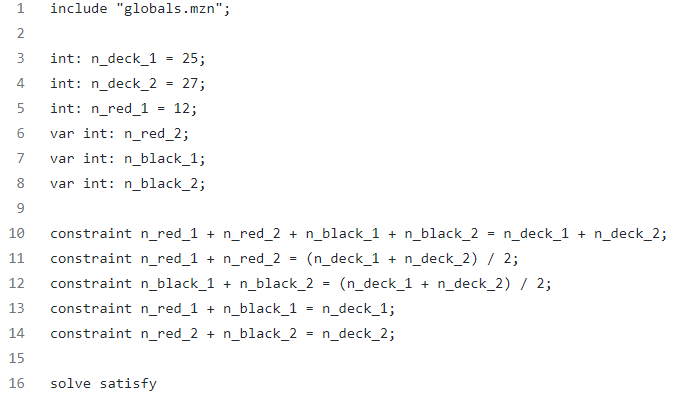
\includegraphics[width=12cm]{img/Es1.png}
\vspace{0.2cm}

The task was to compute the number of black cards contained in the second deck, assumed that
the first one contains 12 red cards. In order to generalize the procedure we defined three parameters:
\textit{n\_deck\_1}, \textit{n\_deck\_2}, \textit{n\_reds\_1}, that are respectively the number of cards in
the first deck, the number of cards in the second deck and the number of red cards in the first deck.\\
The first constraint tells that the sum of red and black cards of both decks must be equal
to the total number of cards. The second constraint imposes that half of the deck is made
up by red cards, and simmetrically the third constraint does the same as regards black cards.
The last two constraints state that the number of cards of a deck is equal to the sum of
its red and black cards.\\
The result can be read in the variable \textit{n\_black\_2}.

\section{Exercise 2}
\vspace{0.2cm}
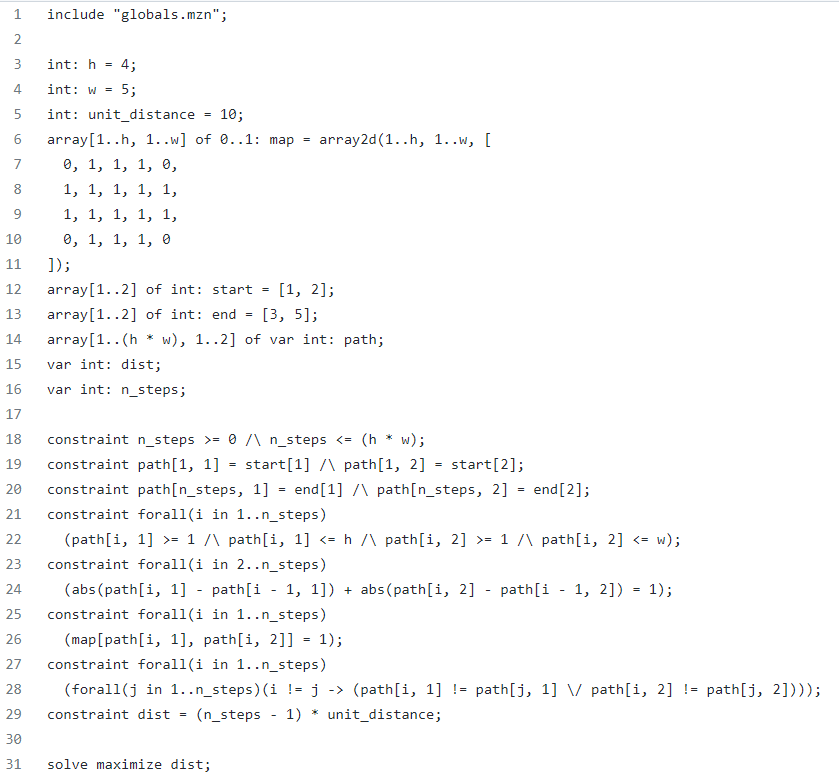
\includegraphics[width=\linewidth]{img/Es2.png}
\vspace{0.2cm}

The grid shown in the figure has been represented through the matrix \textit{map} (whose dimensions has been parametrized
with the variables \textit{h} and \textit{w}), where the ones indicate the presence of a red dot and the zeros its
absence. An additional parameter \textit{unit\_distance} allows to define the distance between two dots 
(set to 10 as required by the exercise).\\
The initial and the final dots of the path have been represented in two arrays of two elements (\textit{start} and \textit{end}), 
each of them storing both the information about the row and the column of the dot.\\
The variable \textit{path} is the sequence of points that are crossed in order to reach the end point from
the start one. It's defined as a two-dimensional array, whose width is equal to the maximum possible number of steps (\textit{h} * \textit{w}) 
and whose height is 2 (each point is described by two coordinates).\\
The variable \textit{dist} is the most relevant of the program and is indeed the one that is maximized to produce the output.
It's defined as the number of steps times the \textit{unit\_distance}.

The second and the third constraints impose that first item of the path is the \textit{start} point and the last item of
the path is the \textit{end} point. 
The fourth constraint ensures that the computed coordinates of the points in the path are inside the range defined
by the size of the grid. The next one formalizes the constraint that each move can be either a unitary horizontal or vertical step.
To be sure that the path doesn't include the points of the grid that are not available, we introduced the fifth constraint,
that checks the values in the \textit{map} array.
The constraint at line 27 imposes that a point is crossed at most once.

\section{Exercise 3}
\vspace{0.2cm}
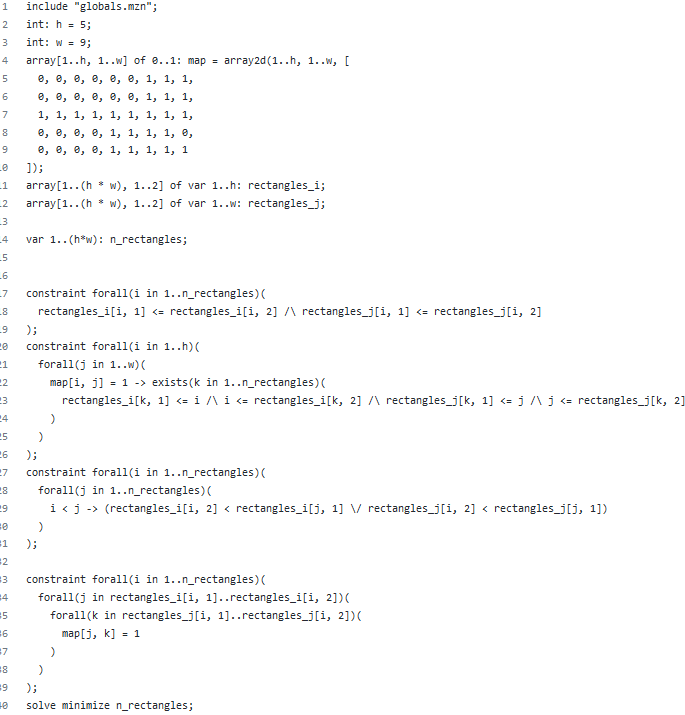
\includegraphics[width=\linewidth]{img/Es3.png}
\vspace{0.2cm}

In order to represent the scheme, we imagined to put a grid over it, to split
the figure in squares. Therefore, we stored it as a matrix, in which a one means that the cell
is part of the drawing and a zero stands for an empty space.
The idea on which the implementation has been based, is about finding the minimum number of rectangles
that can be fit into the figure in order to cover its whole surface. Each internal rectangle is described
by the top-left and bottom-right corners coordinates, stored in two respective arrays: \textit{rectangles\_i} contains
the \textit{i-th} coordinate of both points, whereas \textit{rectangles\_j} is used to store their \textit{j-th} coordinate
(indeed both arrays have 2 as second dimension size). Finally, \textit{n\_rectangles} is the target variable to be minimized.

The first constraint states that for each internal rectangle, the coordinates of the top-left corner must be less than
or equal to the coordinates of the corresponding bottom-right corner.
The second constraint formalizes the concept for which every point of the figure (therefore whose corresponding cell of matrix
\textit{map} has value 1) must be contained into one of the rectangles that have been found.
The third constraint simply ensures that the internal rectangles don't overlap (assuming an ordering among the rectangles
for speed purposes).
The last constraint, checks that every rectangle that has been found actually is a rectangle and there are no holes inside of it, 
so that every point contained between the top-left and the bottom-right corner is part of the drawing.

\section{Exercise 4}
\vspace{0.2cm}
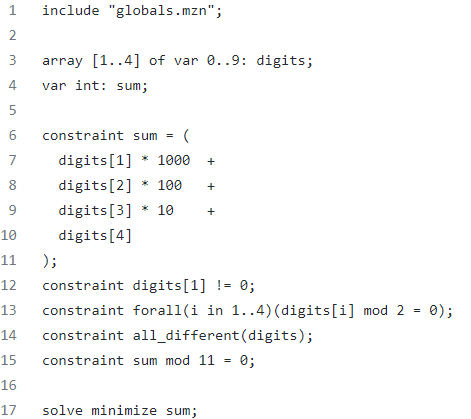
\includegraphics[width=9cm]{img/Es4.png}
\vspace{0.2cm}

In order to implement the constraint related to the fact that every digit of the number must be different,
we represented the number as an array (\textit{digits}), in which the \textit{i-th} position contains the \textit{i-th} digit.
The relation between the array of digits and the number is obtained through the weighted sum of the digits (in 
the variable \textit{sum}).

The constraints simply formalize straightforwardly the requirements of the exercise. Since the goal of the exercise
is to find the smallest number satisfying the constraints, we minimized the value of \textit{sum}.

\section{Exercise 5}
\vspace{0.2cm}
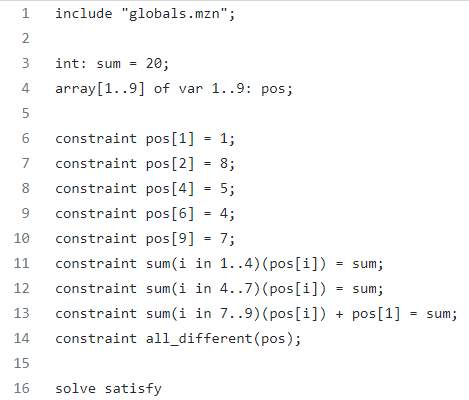
\includegraphics[width=9cm]{img/Es5.png}
\vspace{0.2cm}

The exercise has been parametrized according to the sum of the internal cells of the triangle, defined
in the parameter \textit{sum}. The values of the triangle have been represented with an array (\textit{pos}),
that reflects the cells of the figure, starting from the top and in clockwise order.
The right edge of the triangle is made up by the first four cells, the bottom edge refers to the sum of the
\textit{4-th}, \textit{5-th}, \textit{6-th} and \textit{7-th} cells, and finally the left edge is composed of
the last three positions of the array along with the first one.

\section{Exercise 6}
\vspace{0.2cm}
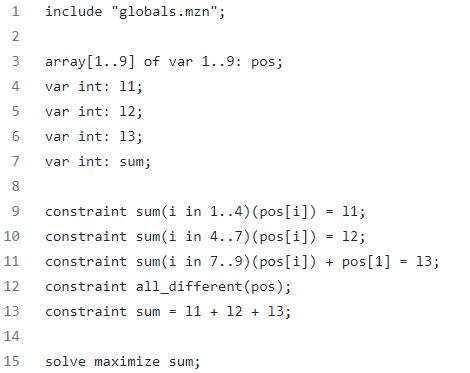
\includegraphics[width=9cm]{img/Es6.png}
\vspace{0.2cm}

The representation of the triangle is the same as the one explained in the Exercise 5. The only
difference is the introduction of the variable \textit{sum}, defined as the sum of the values of 
all the edges (and the value of the edge is computed as previously explained).
The target is no longer to find a set of suitable values, but to maximize the value of the \textit{sum}.

\section{Exercise 7}
\vspace{0.2cm}
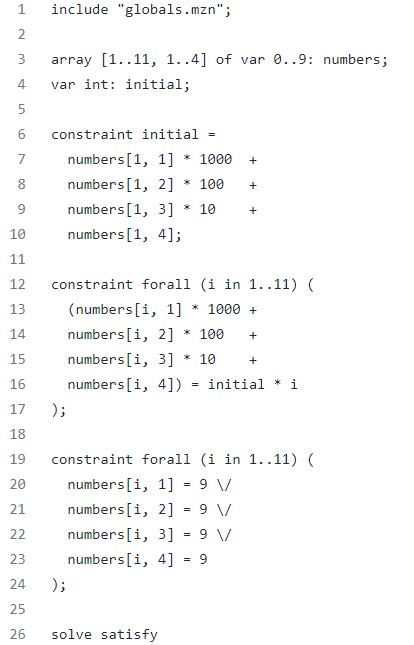
\includegraphics[width=8cm]{img/Es7.png}
\vspace{0.2cm}

In order to deal easily with the digits of the numbers, each number is represented with a 4-elements
array. All the numbers of the sequence (the 11 multiples) are grouped into a unique array (\textit{numbers}),
whose size is therefore 11 x 4. The \textit{i-th} row contains the digits of the \textit{i-th} multiple of
the intial number. 

The matching between the \textit{i-th} row and the corresponding number is formalized through
the second constraint. 
Since the goal is to discover which was the initial number, this is defined in the variable
\textit{initial}, that is then constrained to be equal to the weighted sum of the elements of the first
row of the array.
The last constraint imposes that at least one digit of each multiple is equal to 9 (as required by
the exercise).

\section{Exercise 8}
\vspace{0.2cm}
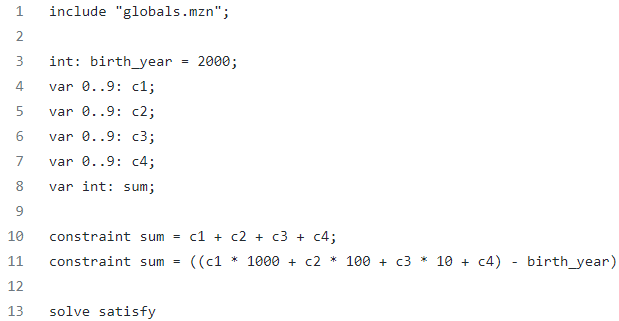
\includegraphics[width=12cm]{img/Es8.png}
\vspace{0.2cm}

We used four variables, one for each digit of the number representing the year, so that the variable
\textit{$c_i$} contains the value of the \textit{i-th} digit. 

The two constraints are trivial, and simply formalize the requirements of the exercise.

\section{Exercise 9}
\vspace{0.2cm}
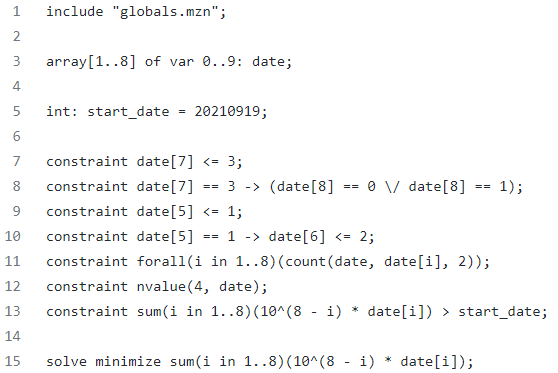
\includegraphics[width=11cm]{img/Es9.png}
\vspace{0.2cm}

Since a date is made up by 8 digits (2 for the day, 2 for the month and the last 4 for the year),
it's been represented with an array of 8 elements. To achieve an ordering, we found it more convenient
to invert the parts of the date, and so we put first the year, followed by the month and the day.
The initial date has been expressed as a number, obtained by the weighted sum of its digits.

The first four constraints simply force the array to represent a semantically valid date.
The fifth constraint states that each digit is present only once in the array. This is checked
by taking advantage of the function \textit{count/3}. The next constraint makes use of the MiniZinc
function \textit{nvalue/2}, that tests if the first parameter is equal to the number of distinct values inside an array.
The last constraint simply ensures that the date produced as output follows the initial one.

\section{Exercise 10}
\vspace{0.2cm}
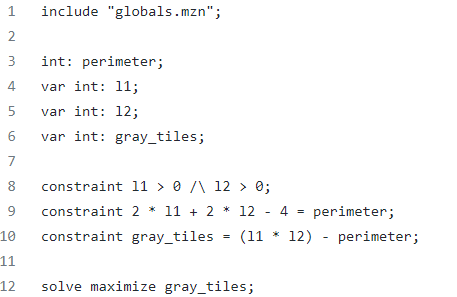
\includegraphics[width=9cm]{img/Es10.png}
\vspace{0.2cm}

In order to generalize the problem, the number of tiles of which the perimeter is made up by is represented
as parameter. Note that the gray tiles can be computed as the area of the rectangle minus the perimeter.
The variables of the problem are the length of the two edges of the rectangle (\textit{l1} and \textit{l2})
and the number of gray tiles (\textit{gray\_tiles}).

In the second constraint, whose target is to express the perimeter as a function of the edges, we subtract 4
because otherwise the corners would be considered twice into the sum. 
The last constraint defines the internal area, and therefore the number of gray tiles, in the previously explained
way.

\section{Exercise 11}
\vspace{0.2cm}
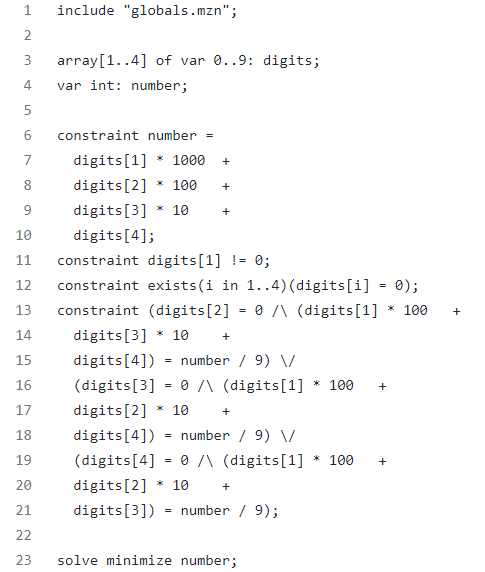
\includegraphics[width=10cm]{img/Es11.png}
\vspace{0.2cm}

The task was to find the smallest 4 digits number such that if we delete a 0 we obtain a ninth of the number itself. \\
Also in this case we represented the number as a 4 dimensional array and we used a constraint to prevent the first digit from being 0, because otherwise the number of digits would be only 3. The other two constraints impose that at least a digit is 0 and they take in consideration the three possible positions of the digit 0: for each possible position they require the weighted sum of the other three digits to be the ninth of the original number.

\section{Exercise 12}
\vspace{0.2cm}
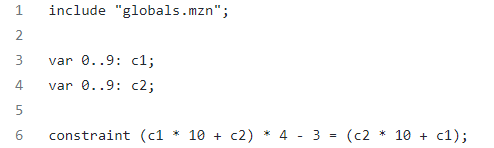
\includegraphics[width=10cm]{img/Es12.png}
\vspace{0.2cm}

In this exercise we represent a 2 digits number with two variables \textit{$c_1$}
and  \textit{$c_2$} and we used a simple constraint to impose that if we multiply the number by 4 and we subtract 3 the resulting number has the same digits of the original number, but in different order.

\section{Exercise 13}
\vspace{0.2cm}
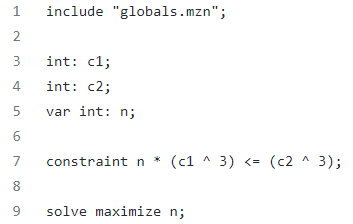
\includegraphics[width=7.5cm]{img/Es13.png}
\vspace{0.2cm}

We used two variables \textit{$c_1$} and \textit{$c_2$} to represent the edges of two cubes and a variable \textit{n} that represent the number of times that the greatest cube can contain the smallest one. We maximized \textit{n}.
The biggest edge is \textit{$c_2$} and \textit{$c_1$} is then the smallest one.

\section{Exercise 14}
\vspace{0.2cm}
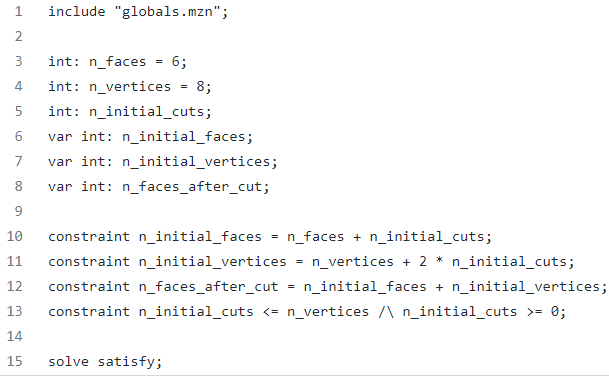
\includegraphics[width=12cm]{img/Es14.png}
\vspace{0.2cm}

We have a cube, and we make a cut around one of its vertices. The task was to find the number of faces of the solid if we perform a cut on 
each of its vertices. 
To express the relation between the number of faces and the number of vertices, we found out that every cut around a vertex introduces an additional
face and two new vertices.

We pursued the goal of making the problem as parametrized as possible, indeed we introduced a parameter \textit{n\_initial\_cuts}
that allows to change the number of cuts that have been performed on the cube before computing the main task.

For these reasons, the first constraint computes the number of faces at the beginning of the execution as 
the sum of the faces of the solid (without any cuts) and the number of cuts already performed (since every cut introduces a new face).
The second constraint is related to the same concept, but as regards the number of vertices.
Since the final number of faces depends on the initial number of faces and the initial number of corners,
we define it as their sum, in the variable \textit{n\_faces\_after\_cut}.

\section{Exercise 15}
\vspace{0.2cm}
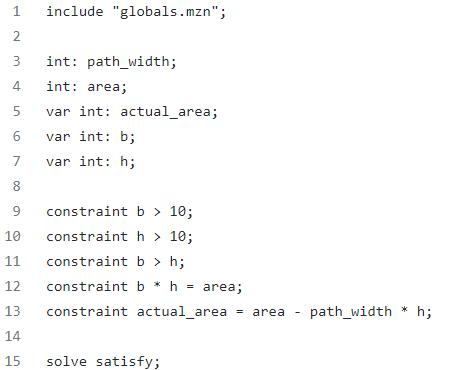
\includegraphics[width=9.5cm]{img/Es15.png}
\vspace{0.2cm}

In this exercise we have to find the area of a portion of a rectangle. Our intuition is that the area of the path can be computed as it was a parallelogram. We use the variable \textit{path\_width} to store the length of the base of the path and two variables \textit{b} and \textit{h} to store the parallelogram dimensions. We used a simple constraint to impose that the remaining area is the area of the total rectangle minus the area of the path.

\section{Exercise 16}
\vspace{0.2cm}
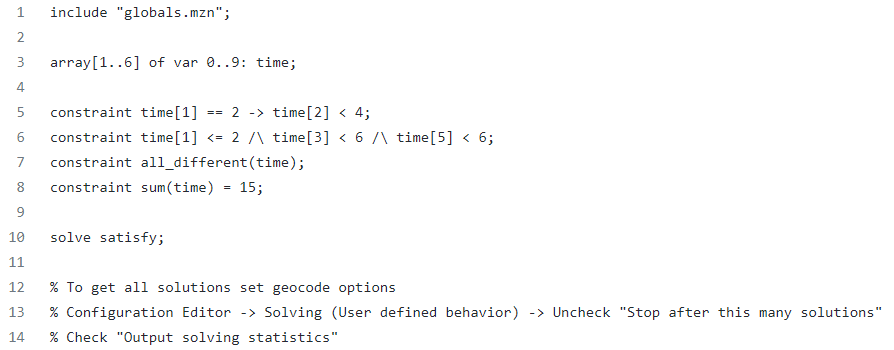
\includegraphics[width=15cm]{img/Es16.png}
\vspace{0.2cm}

The task was to find the number of times that an alarm indicates simultaneously the numbers 0,1,2,3,4,5. We imposed some constraints to construct a realistic hour, for example imposing that the first digit cannot be higher than 2. Then we imposed that the sum of all the digits must be 15, that is the sum of  0,1,2,3,4,5 and that they must be all different.

\section{Exercise 17}
\vspace{0.2cm}
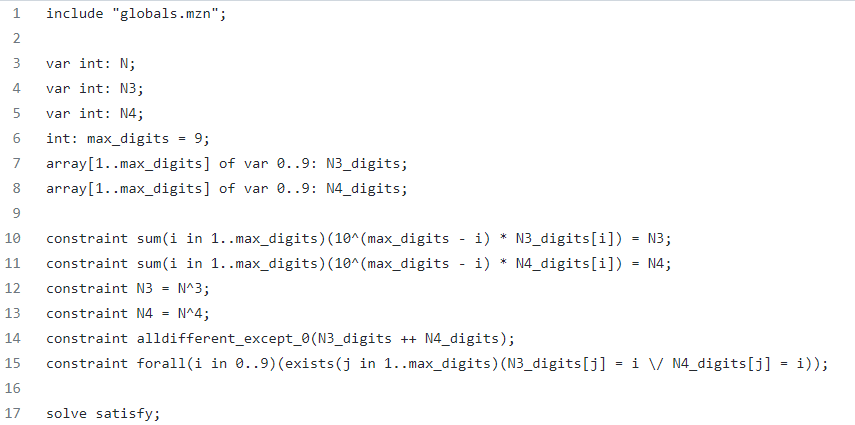
\includegraphics[width=\linewidth]{img/Es17.png}
\vspace{0.2cm}

The task is to find an integer and positive number $N$ such that we have to use all the ten digits to write $N^3$ and $N^4$. 
We used three integer variables to store the values of \textit{N}, \textit{$N_3$} and \textit{$N_4$}
and the digits of $N^3$ and $N^4$ are stored in two arrays \textit{N3$\_$digits} and \textit{N4$\_$digits}. The first constraints impose that the weighted sum of \textit{N3$\_$digits} and \textit{N4$\_$digits} are respectively equal to the numbers \textit{N3} and \textit{N4}. The other constraints impose that the digits in \textit{N3$\_$digits} and \textit{N4$\_$digits} must be all different except for the zero digits, because the two arrays contain 10 elements, therefore there will be more than one element equal to 0. The last constraint imposes that each digit has to appear at least once either in \textit{N3$\_$digits} or in \textit{N4$\_$digits}.

\section{Exercise 18}
\vspace{0.2cm}
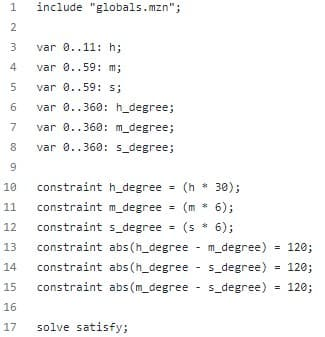
\includegraphics[width=8cm]{img/Es18.jpg}
\vspace{0.2cm}

The task is to find the number of times in which the clock hands form an equilateral triangle. We used three variables to store the hours, the minutes and the seconds and other three variables to store the angles that the three clock hands form with the vertical axis.\\ We used three simple constraints to impose the differences between the angles to be 120, because if the resulting triangle is equilateral the corners in the center must be all equal ($360:3 = 120$).
\end{document}